\documentclass[reprint,english,notitlepage]{revtex4-1}
% if you want a single-column, remove reprint

% allows special characters (including æøå)
\usepackage[utf8]{inputenc}
\usepackage [norsk]{babel} %if you write norwegian
%\usepackage[english]{babel}  %if you write english


\usepackage{physics,amssymb}  % mathematical symbols (physics imports amsmath)
\usepackage{graphicx}         % include graphics such as plots
\usepackage{xcolor}           % set colors
\usepackage{hyperref}         % automagic cross-referencing (this is GODLIKE)
\usepackage{tikz}             % draw figures manually
\usepackage{listings}         % display code
\usepackage{subfigure}        % imports a lot of cool and useful figure commands
\usepackage{float}			  % force placement of tables and figures
\usepackage{amsmath}
\usepackage{minted}

\hypersetup{ % this is just my personal choice, feel free to change things
	colorlinks,
	linkcolor={red!50!black},
	citecolor={blue!50!black},
	urlcolor={blue!80!black}}

%% Defines the style of the programming listing
%% This is actually my personal template, go ahead and change stuff if you want
\lstset{ %
	inputpath=,
	backgroundcolor=\color{white!88!black},
	basicstyle={\ttfamily\scriptsize},
	commentstyle=\color{magenta},
	language=Python,
	morekeywords={True,False},
	tabsize=4,
	stringstyle=\color{green!55!black},
	frame=single,
	keywordstyle=\color{blue},
	showstringspaces=false,
	columns=fullflexible,
	keepspaces=true}

\begin{document}
	
\title{Simulering av Solsystemet med Velocity Verlet Algoritmen \\
	\normalsize FYS4150 - Prosjekt 3}
\date{\today}               
\author{Karl Henrik Fredly}
\affiliation{Universitetet i Oslo} 

\newpage
	
\begin{abstract} %------------------Abstract-----------------------
	I dette prosjektet skal vi simulere solsystemet med Velocity Verlet algoritmen. Vi finner at algoritmen gir et mer riktig resultat enn Euler metoden selv med færre datapunkter. Videre skal vi se på hvordan endring av formelen for tyngdekraften endrer systemet vårt. Vil vil her finne at selv små endringer fra den kjente formelen fører til et ustabilt system.
	
	Vi skal undersøke effekten planetene i solsystemet har på Jordas bane over 100 år. Vi finner at de har en liten, men synlig effekt i figurene våre.
	
	Vi skal se at Velocity Verlet algoritmen lar oss bergne unnslipningshastigheten til jorda på 8.88 AU/yr. Vi gjør et grovt estimat på unnslipningshastigheten og finner at den er mellom 8.8 og 8.9 AU/yr. Til slutt beregner vi også perihelionvinkelen til Merkur over 100 år med relativistisk tyngdekraft på 43'' med god nøyaktighet, vi finner en perihelion vinkel på 55.73''.
	
	- Github repository link med all kode og resultater med ekstra forklaringer: \href{https://github.com/KarlHenrik/ComputationalPhysicsMaster/tree/master/FYS4150/Project3}{https://github.com/KarlHenrik/ComputationalPhysicsMaster/tree/master/FYS4150/Project3}
\end{abstract}
\maketitle

\section{Introduksjon} %------------------Introduksjon-----------------------
	Løsninger av ordinære differensiallikninger er et kraftig verktøy i simuleringen og utforskingen av blant annet fysiske systemer. Velocity Verlet algoritmen er et populært valg av løsere av denne typer ligninger. Vi skal sammenligne Velocity Verlet algoritmen med Euler metoden og videre bruke Velocity Verlet algoritmen til å utforske planetbaner og tyngdekraften.
	
	I metoder seksjonen skal vi utlede Velocity Verlet algoritmen og Euler metoden. Så skal vi vise noen resultater rundt tyngdekraften som Jordens unnslipningshastighet, og at Keplers 2. lov fører til bevaring av angulærmoment. Etterfulgt av en presentasjon av presesjonen til Merkurs perihelion, som vi skal undersøke.
	
	I resultater seksjonen skal vi presentere simuleringer av Jordens bane rundt sola, simulert med Euler metoden og Velocity Verlet algoritmen. Så viser vi simuleringer av det samme systemet med ulike former av tyngdekraften, for å vise hvordan de påvirker stabiliteten til systemet. Videre gjør vi en grov estimering av Jordens unnslipningshastighet. Så viser vi hvordan andre planeter påvirker Jordas bane, før vi presenterer perihelion presesjonen til Merkur vi simulerte.
	
	Til slutt ser vi på hvor gode simuleringene våre var, og hva de forteller oss om tyngdekraften og planetbaner i diskusjonen og konklusjonen.

\section{Metoder} %------------------Metoder-----------------------
	
	
\subsection{Velocity Verlet Algoritmen}
	Vi skal i hovudsak bruke Velocity Verlet algoritmen i simuleringene våre. Utledningen av den er som følger.
	
	Taylor ekspansjonene til posisjon og hastighet er gitt ved
	\begin{equation}
	\label{eq:taylor}
	\begin{aligned}
	&x_{i+1} = x_i + h v_i + \frac{h^2}{2}a_i + O(h^3) \\
	&v_{i+1} = v_i + h a_i + \frac{h^2}{2}a_i' + O(h^3)
	\end{aligned}
	\end{equation}
	hvor $a = v' = x''$. Deriverer vi Taylor ekspansjonen til hastighet får vi
	\begin{equation*}
	\begin{aligned}
	&a_{i+1} = a_i + h a_i' + O(h^3)
	\end{aligned}
	\end{equation*}
	Vi kan dermed tilnærme
	\begin{equation*}
	\begin{aligned}
	&ha_{i}' \approx a_{i + 1} - a_i
	\end{aligned}
	\end{equation*}
	Og vi får da følgende uttrykk for posisjon og hastighet
	\begin{equation*}
	\begin{aligned}
	&x_{i+1} = x_i + hv_i + \frac{h^2}{2}a_i + O(h^3) \\
	&v_{i+1} = v_i + \frac{h}{2}(a_{i+1} + a_i) + O(h^3)
	\end{aligned}
	\end{equation*}
	$h, h/2$ og $h^2/2$ kan regnes ut en gang for alle tidssteg, så hvert tidssteg bruker 8 FLOPs. Det er også verdt å vite at metoden bevarer energi \cite{energi}
	
\subsection{Euler Metoden}
	Vi skal sammenligne Velocity Verlet metoden med Euler Metoden for å se hvor mye det gagner oss å bruke Velocity Verlet metoden. Euler Metoden kommer rett fra ligning \ref{eq:taylor}, hvis vi lar $O(h^2)$ leddene være del av feilen vår.
	\begin{equation}
	\begin{aligned}
	&x_{i+1} = x_i + h v_i + O(h^2) \\
	&v_{i+1} = v_i + h a_i + O(h^2)
	\end{aligned}
	\end{equation}
	Vi ser at hvert tidssteg bruker 4 FLOPs. Metoden bruker altså halvparten så mange FLOPs som Velocity Verlet, men prisen er en større feil, og at Euler Metoden ikke bevarer energi.
	
\subsection{Gravitasjonskraften og Planetbaner}
	Gravitasjonskraften mellom to legemer med masse $M_1$ og $M_2$ og avstand mellom seg $r$ er gitt ved
	\begin{equation}
	\begin{aligned}
	F_G = \frac{GM_1M_2}{r^2}
	\end{aligned}
	\end{equation}
	hvor $G$ er gravitasjonskonstanten. I solsystemet virker denne kraften mellom alle par av objekter som planeter, måner, asteroider og solen. Dette gjør at for N objekter må man regne ut kraften $O(N^2)$ ganger. Vi kommer kun til å holde oss til planetene og solen i solsystemet, så dette blir ikke et stort problem her.
	
	Tyngdekraften er en konservativ kraft. Dette vil si at energien til et legeme i et gravitasjonsfelt er konstant. Når et legeme er langt unna f.eks sola har det mye potensiell energi, og når det faller mot sola blir noe av denne energien gjort om til like mye kinetisk energi. Hvis en planet er i en sirkelbane rundt sola vil både kinetisk og potensiell energi være konstant siden avstanden til sola og planetens hastighet er konstant.
	
	Jorda går i en sirkelbane rundt sola hvis den har en hastighet på $2\pi AU/year$ i en avstand $1 AU$ fra sola, siden hastigheten i en sirkelbane er gitt ved
	\begin{equation}
	\begin{aligned}
	\frac{v^2}{r} = a = \frac{GM_{Sun}}{r^2} \Rightarrow v = \sqrt{\frac{GM_{Sun}}{r}} \approx 2\pi
	\end{aligned}
	\end{equation}
	når r = $1 AU$.
	
	
	Vi skal se på hva unnslipningshastigheten for å unnslippe sola er når man er 1AU unna den. Energien som må til for å dra fra $r=1AU$ til evig langt unna sola er
	\begin{equation}
	\begin{aligned}
	\int_{r}^{\infty}\frac{GM_{Sol}m}{r^2}dr = [-\frac{GM_{Sol}m}{r}]_r^\infty = \frac{GM_{Sol}m}{r}
	\end{aligned}
	\end{equation}
	Vi finner da den nødvendige hastigheten ved å sette den kinetiske energien til legemet lik den nødvendige energien for å unnslippe
	\begin{equation}
	\label{eq:unn}
	\begin{aligned}
	&\frac{1}{2}m v^2  = \frac{GM_{Sol}m}{r} \\
	&v = \sqrt{\frac{2GM_{Sol}}{r}} = 42.1 km/s = 8.88AU/yr
	\end{aligned}
	\end{equation}
	
	Vi skal også se at angulærmomentet til et legeme i bane rundt sola er konstant. Dette følger av Keplers 2. lov som sier at linjen mellom en planet og sola alltid beveger seg over det samme arealet over like tidsrom.
	
	Hvis f.eks Jorda er en avstand $r$ unna sola og beveger seg en vinkel $d\theta$ vil linjen mellom Jorda og sola omtrent bevege seg over en trekant med grunnlinje $r$ og høyde $rd\theta$. Arealet per tidsenhet blir da
	\begin{equation}
	\begin{aligned}
	\frac{dA}{dt} = \frac{1}{2}r r \frac{d\theta}{dt} = \frac{1}{2}r v_{\theta}
	\end{aligned}
	\end{equation}
	Hvor $v_{\theta}$ er vinkelhastigheten til jorda rundt sola. Størrelsen til angulærmomentet til jorda rundt sola er gitt ved
	\begin{equation}
	\begin{aligned}
	L = |m(\vec{r} \cross \vec{v})| = mrv_\theta = 2 m \frac{dA}{dt}
	\end{aligned}
	\end{equation}
	Siden massen er konstant, og Keplers 2.lov sier at $\frac{dA}{dt}$ er konstant vet vi at L også er konstant.
	
\subsection{Perihelion Presesjonen til Merkur}
	Generell relativitetsteori fører til et ekstra ledd i formelen for tyngdekraften som gjør at vi for f.eks sola og Merkur får
	\begin{equation}
	\begin{aligned}
	F_G = \frac{GM_\mathrm{Sol}M_\mathrm{Merkur}}{r^2}\left[1 + \frac{3l^2}{r^2c^2}\right]
	\end{aligned}
	\end{equation}
	hvor $l$ er størrelsen til Merkurs angulærmoment per masseenhet og $c$ er lysets hastighet i vakuum. Dette har en veldig liten effekt på bevegelsen til planetene, men nok til at det over tid er målbart. Hvis vi kun ser på et system med Sola og Merkur vil vi f.eks forvente å se at perihelion vinkelen til Merkur endrer seg med 43'' (arc sekunder) etter 100 år. Perihelion er punktet hvor Merkur er nærmest sola, ellipsebanen til Merkur vil altså bli vridd en liten vinkel.
	

\section{Resultater} %------------------Resultater-----------------------
	Vi har simulert mange ulike planetbaner rundt solen med ulike metoder, ulik tyngdekraft og ulike planeter. Solen holdes i ro i alle simuleringene hvor det motsatte ikke nevnes i figurteksten, slik at vi kan skille mellom variasjoner i baner rundt sola som kommer av simuleringen vår, og som kommer av solas bevegese.

\subsection{Stabiliteten til Euler og Velocity Verlet}
	Vi simulerte jordas ''sirkelbane'' over 10 år med både Euler metoden og Velocity Verlet algoritmen. Banen bør bli en lukket sirkelbane med bevart kinetisk og potensiell energi som vi ser i figur \ref{fig:euler5}, \ref{fig:euleren5}, \ref{fig:vverlet4} og \ref{fig:vverleten4}.
	
	Forskjellen mellom metodene for samme store steglengde ser vi i figur \ref{fig:euler2}, \ref{fig:euleren2}, \ref{fig:vverlet2} og \ref{fig:vverleten2}.
	\begin{figure}[H]
		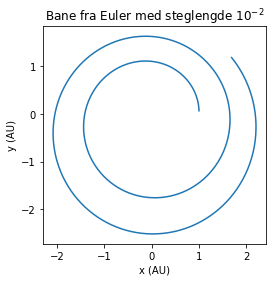
\includegraphics[width=70mm]{../../Code/Figures/euler2.png}
		\caption{Jordas bane rundt sola simulert med Euler Metoden med en steglengde $10^{-2}$ over 5 år.}
		\label{fig:euler2}
	\end{figure}

	\begin{figure}[H]
		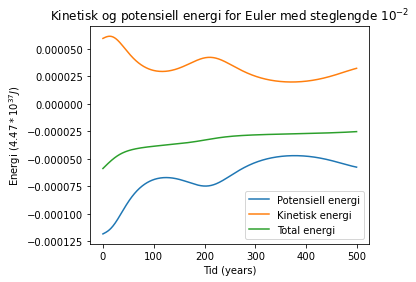
\includegraphics[width=80mm]{../../Code/Figures/euleren2.png}
		\caption{Energien til jorda i bane rundt sola simulert med Euler Metoden med en steglengde $10^{-2}$ over 5 år.}
		\label{fig:euleren2}
	\end{figure}

	\begin{figure}[H]
		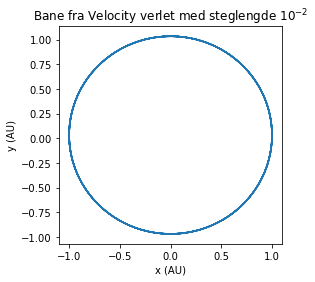
\includegraphics[width=70mm]{../../Code/Figures/vverlet2.png}
		\caption{Jordas bane rundt sola simulert med Velocity Verlet metoden med en steglengde $10^{-2}$ over 5 år.}
		\label{fig:vverlet2}
	\end{figure}
	
	\begin{figure}[H]
		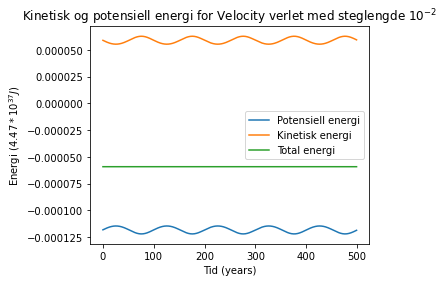
\includegraphics[width=80mm]{../../Code/Figures/vverleten2.png}
		\caption{Energien til jorda i bane rundt sola simulert med Velocity Verlet metoden med en steglengde $10^{-2}$ over 5 år.}
		\label{fig:vverleten2}
	\end{figure}

	\begin{figure}[H]
		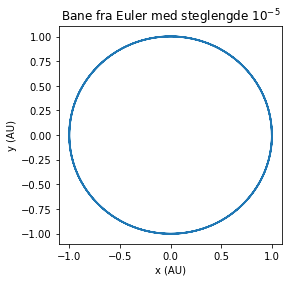
\includegraphics[width=70mm]{../../Code/Figures/euler5.png}
		\caption{Jordas bane rundt sola simulert med Euler Metoden med en steglengde $10^{-5}$ over 5 år.}
		\label{fig:euler5}
	\end{figure}
	
	\begin{figure}[H]
		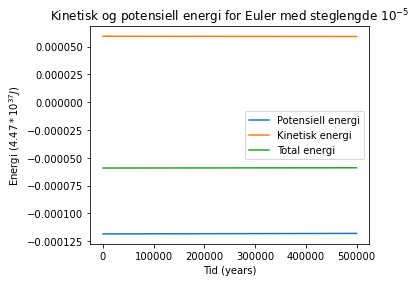
\includegraphics[width=80mm]{../../Code/Figures/euleren5.png}
		\caption{Energien til jorda i bane rundt sola simulert med Euler Metoden med en steglengde $10^{-5}$ over 5 år.}
		\label{fig:euleren5}
	\end{figure}

	\begin{figure}[H]
		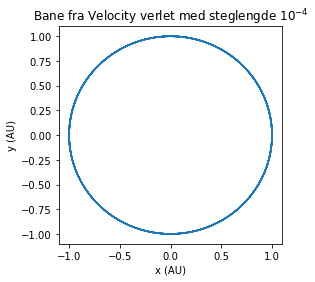
\includegraphics[width=70mm]{../../Code/Figures/vverlet4.png}
		\caption{Jordas bane rundt sola simulert med Velocity Verlet metoden med en steglengde $10^{-4}$ over 5 år.}
		\label{fig:vverlet4}
	\end{figure}
	
	\begin{figure}[H]
		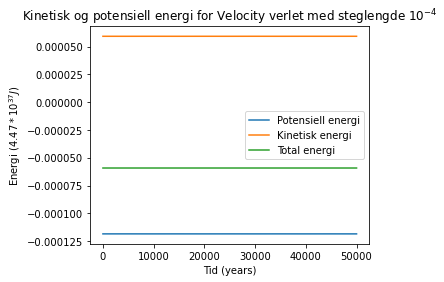
\includegraphics[width=80mm]{../../Code/Figures/vverleten4.png}
		\caption{Energien til jorda i bane rundt sola simulert med Velocity Verlet metoden med en steglengde $10^{-4}$ over 5 år.}
		\label{fig:vverleten4}
	\end{figure}
	Tiden Velocity Verlet og Euler brukte i utregningen av Jordas bane rundt sola med kun de to legemene i simuleringen er vist i tabell \ref{tab:time}.

	\begin{table}[H]
		\begin{center}
			\caption{Tiden Velocity Verlet og Euler brukte for ulike antall punkter med Jorda og sola.}
			\label{tab:time}
			\begin{tabular}{|c|c|c|} \hline
				\textbf{n} & \textbf{Velocity Verlet tid (s)} & \textbf{Euler tid (s)} \\ \hline
				$5*10^5$ & 0.02 & 0.02 \\
				$5*10^6$ & 0.23 & 0.11 \\
				$5*10^7$ & 2.25 & 1.14 \\
				$5*10^8$ & 22.63 & 11.59 \\ \hline
			\end{tabular}
		\end{center}
	\end{table}

\subsection{Ulike eksponenter i tyngdekraften}
	Vi undersøkte om en annen eksponent for $r$ i tyngdekraften endret oppførselen til planetene. Vi kaller eksponenten $\beta$ slik at tyngdekraften blir gitt ved
	\begin{equation}
	\begin{aligned}
	F_G = \frac{GM_1M_2}{r^\beta}
	\end{aligned}
	\end{equation}
	Vi såg først på effekten av ulike eksponenter for en Jordas sirkelbane, vist i figur \ref{fig:betacirc}. Energi og angulærmoment var her så godt som bevart for alle eksponenter, siden Jorda bare holder seg i en sirkelbane.

	\begin{figure}[H]
		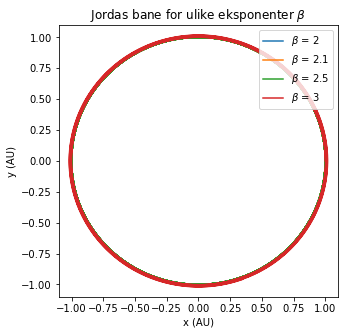
\includegraphics[width=80mm]{../../Code/Figures/betacirc.png}
		\caption{Jordas bane rundt sola simulert med Velocity Verlet metoden med en steglengde $10^{-4}$ over 10 år for ulike eksponenter for $r$ i tyngdekraften. Starter med initialbetingelser for sirkulær bane.}
		\label{fig:betacirc}
	\end{figure}

	Videre såg vi hva endring av eksponenten hadde å si når Jorda var i en ellipsebane, vist i figure \ref{fig:betaell}.

	\begin{figure}[H]
		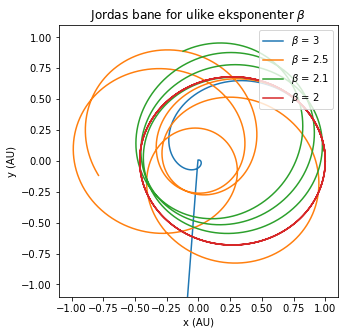
\includegraphics[width=80mm]{../../Code/Figures/betaell.png}
		\caption{Jordas bane rundt sola simulert med Velocity Verlet metoden med en steglengde $10^{-4}$ over 10 år for ulike eksponenter for $r$ i tyngdekraften. Starter med initialbetingelser for elliptisk bane.}
		\label{fig:betaell}
	\end{figure}
	Hvordan energien og angulærmomentet til systemet endrer seg for valget av eksponent $\beta = 2.5$ ser vi i figur \ref{fig:betaen} og \ref{fig:betaang}.

	\begin{figure}[H]
		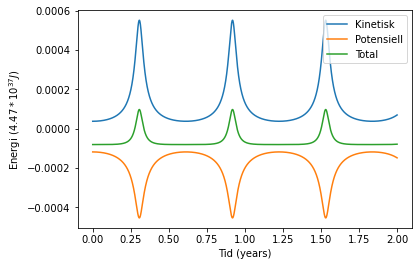
\includegraphics[width=80mm]{../../Code/Figures/betaen.png}
		\caption{Jordas energi i en ellipsebane med eksponent 2.5 for $r$ i tyngdekraften.}
		\label{fig:betaen}
	\end{figure}

	\begin{figure}[H]
		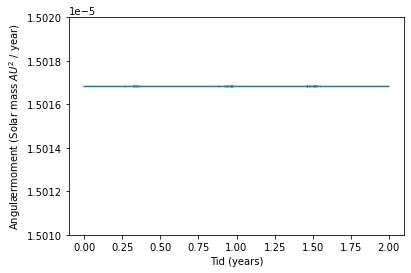
\includegraphics[width=80mm]{../../Code/Figures/betaang.png}
		\caption{Jordas angulærmoment i en ellipsebane med eksponent 2.5 for $r$ i tyngdekraften.}
		\label{fig:betaang}
	\end{figure}

\subsection{Unnslipningshastigheten til Jorda}
	For å undersøke om simuleringen vår stemmer med fysikken såg vi om unnslipningshastigheten til jorda stemte med beregningene våre i ligning \ref{eq:unn}. Vi lar Jorda start i posisjon x = 1AU med med ulike starthastigheter i x-retningen. Hvordan Jordas x-posisjon da endrer seg over 100 år er vist i figur \ref{fig:escape}.

	\begin{figure}[H]
		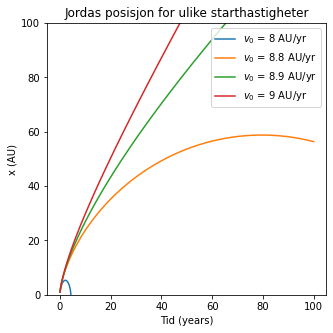
\includegraphics[width=80mm]{../../Code/Figures/escape.png}
		\caption{Jordas x-posisjon over 100 år for ulike startfarter rett ut fra sola. Jorda starter ved 1 AU.}
		\label{fig:escape}
	\end{figure}

\subsection{Flere legemer}
	Vi skal nå se på hvordan introduksjonen av flere legemer påvirker Jordas bane rundt sola. Fra nå av bruker vi ekte data fra NASA\cite{NASA} i bergningene våre.
	
	Figur \ref{fig:j1}, \ref{fig:j10} og \ref{fig:j1000} viser hvordan Jupyter med ulike masser påvirker Jordas bane, og figur \ref{fig:jstat10} viser hvordan Jupyter med 10 ganger sin vanlige masse påvirker Jorda når sola holdes i ro i origo.

	\begin{figure}[H]
		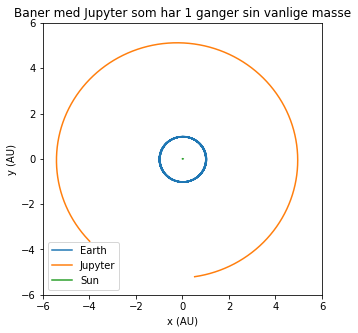
\includegraphics[width=80mm]{../../Code/Figures/j1.png}
		\caption{Jordens og Jupyters posisjon over 10 år med en steglengde på $10^{-4}$. Simulert med Velocity Verlet algoritmen. Solen beveger på seg.}
		\label{fig:j1}
	\end{figure}

	\begin{figure}[H]
		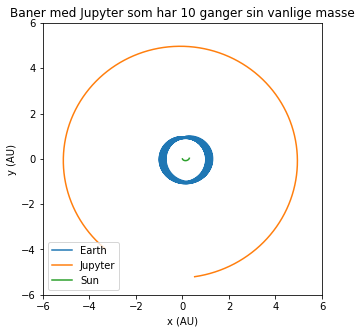
\includegraphics[width=80mm]{../../Code/Figures/j10.png}
		\caption{Jordens og Jupyters posisjon over 10 år med en steglengde på $10^{-4}$. Simulert med Velocity Verlet algoritmen. Jupyter har 10 ganger sin vanlige masse, og solen beveger seg.}
		\label{fig:j10}
	\end{figure}

	\begin{figure}[H]
		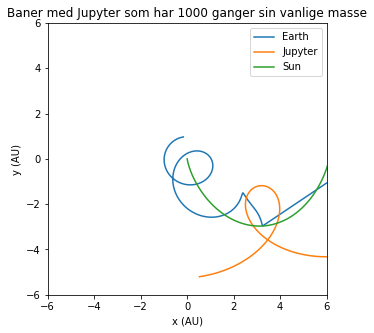
\includegraphics[width=80mm]{../../Code/Figures/j1000.png}
		\caption{Jordens og Jupyters posisjon over 10 år med en steglengde på $10^{-4}$. Simulert med Velocity Verlet algoritmen. Jupyter har 1000 ganger sin vanlige masse, og solen beveger seg.}
		\label{fig:j1000}
	\end{figure}

	\begin{figure}[H]
		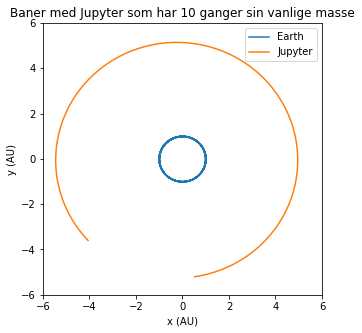
\includegraphics[width=80mm]{../../Code/Figures/jstat10.png}
		\caption{Jordens og Jupyters posisjon over 10 år med en steglengde på $10^{-4}$. Simulert med Velocity Verlet algoritmen. Jupyter har 10 ganger sin vanlige masse, og solen holdes i ro i origo.}
		\label{fig:jstat10}
	\end{figure}

	Figur \ref{fig:all} viser planetbanene når alle planetene er med i simuleringen, og figur \ref{fig:inner} viser utsnittet av samme figur med kun de indre planetene.

	\begin{figure}[H]
		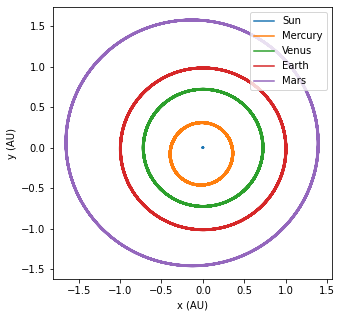
\includegraphics[width=80mm]{../../Code/Figures/inner.png}
		\caption{De indre planetenes posisjon over 100 år med en steglengde på $10^{-4}$. Simulert med Velocity Verlet algoritmen og alle planetene til stede. Solen beveger på seg.}
		\label{fig:inner}
	\end{figure}

	\begin{figure}[H]
		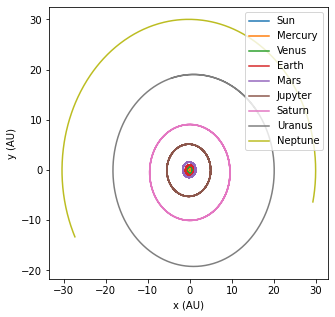
\includegraphics[width=80mm]{../../Code/Figures/all.png}
		\caption{Alle planetenes posisjon over 100 år med en steglengde på $10^{-4}$. Simulert med Velocity Verlet algoritmen. Solen beveger på seg.}
		\label{fig:all}
	\end{figure}

	Figur \ref{fig:100years} viser hvordan Jordas bane over 100 år ser ut med alle planetene med i simuleringen, og med kun Jorda og sola.

	\begin{figure}[H]
		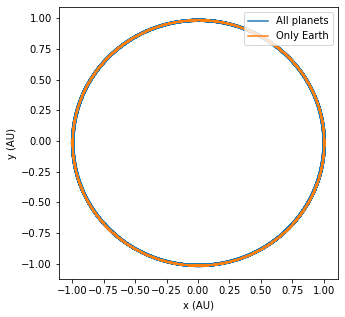
\includegraphics[width=80mm]{../../Code/Figures/100years.png}
		\caption{Jordas posisjon over 100 år med en steglengde på $10^{-4}$. Simulert med Velocity Verlet algoritmen med kun jorda og sola, og med alle de andre planetene. Solen beveger på seg.}
		\label{fig:100years}
	\end{figure}

\subsection{Merkurs Perihelion Presesjon}
	Vi simulerte Merkurs bane rundt sola, med ingen andre planeter til stede i 100 år med 75 millioner punkter, med og uten relativistisk tyngdekraft. Så regnet vi ut perihelion vinkelen til Merkur, eller hvor mye ellipsebanen ble vridd. Vinklene vi fann, og vinkelen vi burde forventet med relativistisk tyngdekraft\cite{oppgave} er vist i tabell \ref{tab:peri}.
	\begin{table}[H]
		\begin{center}
			\caption{Perihelion vinkel for Merkur etter 100 år.}
			\label{tab:peri}
			\begin{tabular}{|c|c|} \hline
				\textbf{} & \textbf{Perihelion Vinkel} \\ \hline
				Forutsett & 43'' \\
				Relativistisk & 55.73'' \\
				Ikke-relativistisk & 0.4330'' \\ \hline
			\end{tabular}
		\end{center}
	\end{table}
	Perihelion til Merkur ved år 0 (her 2020) og år 100 med relativistisk tyngdekraft er vist i figur \ref{fig:peri}. Figuren er veldig zoomet inn siden punktene ikke kan skilles fra hverandre i et plot av hele banen til Merkur.
	\begin{figure}[H]
		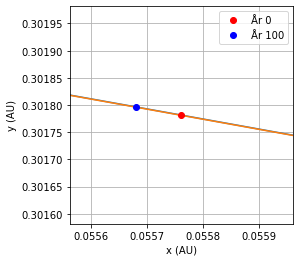
\includegraphics[width=80mm]{../../Code/Figures/peri.png}
		\caption{Forflytning av merkurs perihelion etter 100 år med relativistisk tyngdekraft.}
		\label{fig:peri}
	\end{figure}

	
\section{Diskusjon} %------------------Diskusjon-----------------------

\subsection{Stabiliteten til Euler og Velocity Verlet}
	I figur \ref{fig:euler2} og \ref{fig:euleren2} ser vi at Euler metoden med stor steglengde gjør en dårlig jobb med å bevare energi, siden Jorden beveger seg stadig lengre ut og den totale energien i systemet stadig øker. I figur \ref{fig:vverlet2} ser vi at potensiell og kinetisk energi ikke er helt konstant for velocity verlet metoden heller, men at systemet er stabilt for selv en relativt stor steglengde.
	
	I figur \ref{fig:euler5}, \ref{fig:euleren5}, \ref{fig:vverlet4} og \ref{fig:vverleten4} ser vi at begge metodene gir en sirkelbane med riktig oppførsel, men at velocity verlet ikke trenger en like liten steglengde for å oppnå dette. (Enda flere plot over stabiliteten til metodene finnes i \cite{myRepo})
	
	Denne ekstra nøyaktigheten koster mer tid per simulering, som vist i tabell \ref{tab:time}. Velocity Verlet bruker omtrent dobbelt så lang tid som Euler, og tiden begge tar øker lineært med antall datapunkter. Dette er som vi forventer gitt at Velocity Verlet metoden bruker 8n FLOPs og Euler bruker 4n FLOPs. Feilen i til Velocity Verlet er en faktor $h$ mindre enn feilen i Euler, så det lønner seg dermed nesten alltid å bruke Velocity Verlet algoritmen siden en halvert hastighet er mer enn verdt det.

\subsection{Ulike eksponenter i tyngdekraften}
	I figur \ref{fig:betacirc} ser vi at eksponenten i tyngdekraftleddet kun har en liten påvirkning på sirkelbaner. Men i figur \ref{fig:betaell} ser vi at en elliptisk bane blir endret betydelig når man endrer eksponenten til $r$ i tyngdekraften. For $\beta = 2$ har vi den vanlige ellipsebanen, for $\beta = 2.1$ vrir ellipsebanen seg og for $\beta = 2.5$ blir vridningen ekstrem. For $\beta = 3$ sendes Jorden rett mot solen hvor den blir slengt ut igjen. Siden vi vet fra observasjoner av solsystemet at planetene har stabile ellipsebaner kan vi fastslå at eksponenten til $r$ i tyngdekraften ikke er langt unna 2. For å bli mer sikker på hva eksponenten er, må man gjøre nøyaktige målinger.
	
	Vi valgte å se nærmere på energien og angulærmomentet for ''ellipsebanen'' med $\beta = 2.5$. I figur \ref{fig:betaen} ser vi at energi ikke er bevart, og i figur \ref{fig:betaang} ser vi at angulærmoment fortsatt er bevart. Dette gir mening siden tyngdekraft med $\beta$ ulik 2 ikke er en konservativ kraft, men den påfører fortsatt ikke noe dreiemoment på systemet siden den virker fra origo i systemet i parallelt med posisjonsvektoren til jorda.
	
\subsection{Unnslipningshastigheten til Jorda}
	Figur \ref{fig:escape} viser at unnslipningshastigheten til Jorda ligger i samme område som det analytiske svaret vi fann på 8.88 AU/yr. En starthastighet på 8.9AU/yr ser ut til å føre til at Jorda unnslipper solas tyngdekraft, mens en starthastighet på 8.8AU/yr fører til at Jorda faller tilbake mot sola.

\subsection{Flere legemer}
	Figur \ref{fig:j1} og \ref{fig:j10} viser at Jupyter ikke har noen enorm påvirkning på Jordas bane, men en 10 ganger så massiv Jupyter beveger både sola og Jorda en betydelig mengde. Figur \ref{fig:jstat10} viser at en 10 ganger så massiv Jupyter har relativt lite direkte innvirkning på Jordas bane, og at endringen i jordas bane vi ser i figur \ref{fig:j10} skyldes solas bevegelse. Figur \ref{fig:j1000} viser at en Jupyter med 1000 ganger sin vanlige masse er massiv nok til å i veldig stor grad påvirke både Jorda og sola. Dette er ikke overraskende siden sola kun er omtrent 1000 ganger mer massiv enn Jupyter.

	Figur \ref{fig:all} og \ref{fig:inner} viser at simuleringen vår gir resultater nært det vi forventer for bevegelsen til solsystemet over 100 år. Figur \ref{fig:100years} viser at de andre planetene har en liten, men merkbar påvirkning på Jordas bane over 100 år. Med kun Jorda og sola blir banen mer lukket og veldefinert enn med alle planetene tilstede. Dette ser vi ved at den blå banen til Jorda med alle planetene trekker ut på innsiden og utsiden av den oransje banen med kun Jorda.
	
\subsection{Merkurs Perihelion Presesjon}
	Presesjonensvinkelen vi fann til perihelion for Merkur var 55.73'', mens den vi hadde forventet er 43''. Dette er et så godt resultat vi kunne forventet med begrensningene til metoden og maskinvaren vi jobbet med. Det er også et godt resultat at presesjonsvinkelen uten relativistisk tyngdekraft var 0.4330'', altså to størrelsesordener mindre enn den relativistiske. Vi skulle her forventet 0'', men igjen er dette så godt vi kan forvente. Figur \ref{fig:peri} viser at perihelion til Merkur flytter seg ''mot klokken'', som også stemmer med teorien.

\section{Konklusjon} %------------------Konklusjon-----------------------
	Vi har evaluert simuleringen av solsystemet Velocity Verlet algoritmen gir oss. Vi har sett at den bevarer energien i systemet, og at den gir en god simulering av Jordens bane over 5 år med en steglengde på kun $10^4$, 10 ganger større enn for Euler metoden.
	
	Vi har også sett at de stabile ellipsebanene vi observerer i solsystemet ikke kan være resultatet av en tyngdekraft med $r$ eksponent langt unna 2. Videre fant vi at simuleringer av Jordas unnsliningshastighet samsvarte med vårt analytiske svar på 8.88AU/yr.
	
	Vi observerte at de andre planetene i solsystemet påvirker Jordens bane en liten, men merkbar mengde. En 10 ganger så massiv Jupyter hadde derimot endrer Jordens og solens bane mye.
	
	Til slutt simulerte vi Merkur-Sol systemet i 100 år med 75 millioner punkter og relativistisk tyngdekraft og fikk en perihelion vinkel på 55.73'' som stemmer godt med den forventede perihelion vinkelen på 43''.

\begin{figure*} \bibliography{biblio} \end{figure*}
	
\end{document}